\documentclass[%
 reprint,
superscriptaddress,
groupedaddress,
%unsortedaddress,
%runinaddress,
%frontmatterverbose, 
%preprint,
%preprintnumbers,
%nofootinbib,
%nobibnotes,
%bibnotes,
 amsmath,amssymb,
 aps,
prl,superscriptaddress
%prb,
%rmp,
%prstab,
%prstper,
%floatfix,
]{revtex4-2}

\usepackage{graphicx}% Include figure files
\usepackage{dcolumn}% Align table columns on decimal point
\usepackage{bm}% bold math
\usepackage{braket}
\usepackage{color}
\graphicspath{{./figures/}}
\bibliographystyle{apsrev4-2}

\begin{document}

%\title{Pseudogapped non-Fermi liquid phase arising from Kondo breakdown at the Mott transition}

%\title{Long range entangled Fermi arcs in a Pseudogapped Mott transition}

\title{Pseudogapped Mott criticality: Stretching Kondo Screening to Breaking Point}

%\title{What lies between a Fermi liquid and a Mott insulator in two dimensions? Insights from an impurity model}% Force line breaks with \\

\author{Abhirup Mukherjee}
\affiliation{%
 Department of Physical Sciences, Indian Institute of Science Education and Research Kolkata, Nadia - 741246, India
}
\author{S. R. Hassan}
\affiliation{The Institute of Mathematical Sciences, C.I.T. Campus, Chennai 600 113, India}
\author{Anamitra Mukherjee}
\affiliation{1 School of Physical Sciences, National Institute of Science, Education and Research, HBNI, Jatni 752050, India}
\author{N. S. Vidhyadhiraja}
\affiliation{Theoretical Sciences Unit, Jawaharlal Nehru Center for Advanced Scientific Research, Jakkur, Bengaluru 560064, India}
\author{A. Taraphder}
\affiliation{Department of Physics, Indian Institute of Technology Kharagpur, Kharagpur 721302, India}
%
\author{Siddhartha Lal}
\affiliation{%
 Department of Physical Sciences, Indian Institute of Science Education and Research Kolkata, Nadia - 741246, India
}

\date{\today}
\begin{abstract}
We present an auxiliary model approach that illuminates the centrality of the pseudogap phenomenon in the Mott transition of the Hubbard-Heisenberg model on the half-filled square lattice. Passage from Fermi liquid metal to Mott insulator involves two stages: the first involves a systematic unraveling of Kondo screening due to frustrating charge fluctuations in the conduction bath of the underlying lattice-embedded quantum impurity model. The destabilises the bulk Fermi liquid, culminating in disconnection of the Fermi surface by gapping the antinodes. In the second stage, an emergent pseudogap phase arises from an effective two-channel Kondo problem in the underlying impurity model. The resulting momentum-space Fermi arcs possess non-Fermi liquid excitations proximate to a critical Fermi surface. Upon approaching the transition, the nature of this exotic metal evolves with shrinking size of the arcs towards a singular nodal non-Fermi liquid. This accompanies the onset of long-ranged real-space entanglement and spin-flip correlations, and reveals the Mott transition on the square lattice to be well beyond the paradigm of local quantum criticality.
\end{abstract}

\maketitle

\par\noindent\textit{Introduction.}
The origin of the pseudogap and strange metal phases of the cuprates continue to be hotly debated topics in the context of high-temperature superconductivity~\cite{keimer2015quantum}. The anomalous pseudogap (PG) phase, observed most prominently in the cuprates, exhibits nodal-antinodal dichotomy with spectral weight 
concentrated on Fermi arcs around the nodal regions~\cite{loeserKapitulnik1996,Norman1998,Hashimoto2014}. While several methods have observed a PG in the two dimensional Hubbard model ~\cite{KyungKotliar2006,MacridinAzevedo2006,WuFerrero2018,anirbanmott2,HilleAndergassen2020}, there is no general consensus regarding various aspects of the PG phase, including its relation to proximate Mott insulating and superconducting phases~\cite{FradkinRevModPhys2015,anirbanmott2,Kitatani2023,Sorella2023}, its evolution from weak- to strong-coupling ~\cite{HuangDevereaux2018,Fedor2022,SimkovicFerrero2024}, and whether nodal-antinodal dichotomy is intrinsic to the model~\cite{Hashimoto2014,Schafer2021}. Importantly, the connection between finite-temperature crossovers and zero-temperature ground states observed in various analyses remains unclear~\cite{White1998,Ido2018,ProustTaillefer2019,Ponsioen2019,Shengtao2021,XuZhang2022}.

We present here a new auxiliary model approach 
to the strong coupling physics of the particle-hole symmetric 2D Hubbard-Heisenberg model at zero temperature, revealing the origin and nature of its PG phase and subsequent Mott transition. The first step 
requires identifying an appropriate lattice-embedded quantum impurity model, and conducting a scaling analysis of its low-energy phases. Subsequently, the lattice model is  constructed by applying many-body lattice translation operators~\cite{stoyanova} on the impurity model (referred to henceforth as \textit{tiling}), obtaining thereby various quantities
of the former from the latter. Translation invariance is thus restored differently within our approach from the dynamical mean-field approximation~\cite{georges1996} and its cluster variants~\cite{Hettler2000DCA,Kotliar2001Cellular,Maier2005,Sakai2023}. 

Combining the scaling analysis of the impurity model with the tiling procedure provides the momentum-space resolution crucial to unveiling the PG phenomenon, and clarifies the role of the Kondo breakdown process at the heart of the Mott transition~\cite{fabrizio2017kondophysicsmotttransition,RADEMAKER2025}. Emerging from a systematic unraveling of Kondo screening, the PG phase is separated from Fermi liquid and Mott insulating phases by correlation-driven Lifshitz transitions of the Fermi surface~\cite{sakai2009evolution}. Passage through the PG involves dynamical transfer of spectral weight between gapped anti-nodal Luttinger surfaces (zeros of the single-particle Greens function) and gapless nodal arcs with non-Fermi liquid excitations. We also observe the onset of long-ranged real-space entanglement and spin-flip correlations close to the Mott transition, rendering it beyond the paradigm of local quantum criticality~\cite{Si2001}.  

\par\noindent\textit{A lattice-embedded impurity model.}
Building on insight that Kondo breakdown in a simple extension of the Anderson impurity~\cite{Mukherjee_2023} captures the physics of the Mott transition in infinite dimensions~\cite{georges1996}), we study the Kondo physics of a similar Anderson impurity model embedded within a square lattice 
\begin{equation}\begin{aligned}\label{impurityModel}
	\mathcal{H}_\text{aux} = H_\text{imp} + H_\text{imp-cbath} + H_\text{cbath}~, 
\end{aligned}\end{equation}
where $H_{imp} = - \frac{U}{2}\left(\hat n_{d \uparrow} - \hat n_{d \downarrow} \right) ^2$ is the Hamiltonian for the localised impurity site, and the impurity ($c_{d\sigma}$, with spin-1/2 moment ${\bf S}_d$) 
interacts with four nearest neighbour sites ($c_{Z\sigma}$, labelled with index $Z$) 
through local Kondo terms of uniform strength $J$ as well as single-particle hybridisation $V$, \(H_\text{imp-cbath} =\frac{1}{2} J\sum_{\sigma_1,\sigma_2}\sum_{Z} {\bf S}_d\cdot c^\dagger_{Z\sigma_1}{\boldsymbol \tau}_{\sigma_1,\sigma_2} c_{Z\sigma_2} - V \sum_{\sigma, Z} \left(c^\dagger_{Z\sigma} c_{d\sigma} + h.c.\right)\). Finally, the term
$H_\text{cbath} = \sum_{{\bf k}}\epsilon_{\textbf{k}}
c^\dagger_{{\bf k},\sigma}c_{{\bf k},\sigma} -\frac{W}{2}\sum_{Z} \left(n_{Z\uparrow} - n_{Z\downarrow}\right)^2$ includes the kinetic energy ($\epsilon_{\textbf{k}}=-2t\left(\cos k_x + \cos k_y\right)$) for conduction bath tight-binding electrons ($c^\dagger_{{\bf k},\sigma}$) 
on a half-filled square lattice (with lattice spacing set to unity), together with local correlations ($W$) that frustrate the Kondo screening. The 2D structure of the impurity model, and its distinction from the infinite-dimensional counterpart, becomes apparent upon Fourier transforming the Kondo coupling to ${\bf k}$-space: 
$J_{{\bf k}, {\bf k}^\prime} = \frac{J}{2}\left[\cos\left({\bf k}_x - {\bf k}^\prime_x\right) + \cos\left({\bf k}_y - {\bf k}^\prime_y\right)\right]$, with $J>0$. Clearly, $J_{{\bf k}, {\bf k}^\prime}$ 
possesses the $C_{4}$ lattice symmetry. 
\par\noindent\textit{Reconstructing the lattice model.}
We now define the {\it tiling} procedure by which we recreate the lattice model from the impurity model Hamiltonian. For a {\it unit cell} of the tiling,  
we consider an impurity model \(\mathcal{H}_\text{aux}({\bf r}_d)\) that has the impurity site at a reference site \({\bf r}_d\) of our lattice. In order to create the lattice model, we translate the unit cell across all sites of the lattice:
\begin{equation}\begin{aligned}
	\label{tilingPrescription}
	\mathcal{H}_\text{tiled} &= \sum_{{\bf r}}T^\dagger({\bf r})\mathcal{H}_\text{aux}({\bf r}_d)T({\bf r}) - N\mathcal{H}_\text{cbath},
\end{aligned}\end{equation}
where \({\bf r}\) sums over all lattice sites, and $T({\bf r})$ is a many-body translation operator that translates all coordinates by a vector \({\bf r}\). Further details of the tiling procedure are provided in the Supplemental Material~\cite{suppmat}. Implementing this procedure for the extended Anderson impurity model defined above (eq.~\ref{impurityModel}) generates a {\it Hubbard-Heisenberg} lattice model in two spatial dimensions:
    \begin{eqnarray}
        &&\mathcal{H}_\text{tiled} = -\frac{\tilde t}{\sqrt\mathcal{Z}}\sum_{\left<{\bf r}_i, {\bf r}_j\right>;\sigma}\left(c^\dagger_{{\bf r}_i,\sigma}c_{{\bf r}_j,\sigma} + \text{h.c.}\right) - \tilde \mu \sum_{{\bf r}}\hat n_{{\bf r},\sigma}\nonumber \\
        &&+ \frac{\tilde J}{\mathcal{Z}}\sum_{\left< {\bf r}_i, {\bf r}_j\right>}{\bf S}_{{\bf r}_i}\cdot{\bf S}_{{\bf r}_j} - \frac{1}{2}\tilde U\sum_{\bf r}\left(\hat n_{{\bf r} , \uparrow} - \hat n_{{\bf r} , \downarrow}\right)^2~,
        \end{eqnarray}
with parameters $(\tilde{t},\tilde{\mu},\tilde{J},\tilde{U})$
that are related simply to those in $\mathcal{H}_\text{aux}$~\cite{suppmat}. The form of the eigenstates of $H_{\text{tiled}}$ are dictated by a many-body version of Bloch's theorem~\cite{stoyanova}. Further, relations between the Hamiltonians and eigenstates of the impurity and lattice models are exploited in obtaining equal-time correlation functions and entanglement measures of the latter from the former~\cite{suppmat}.
\begin{figure}
    \centering
    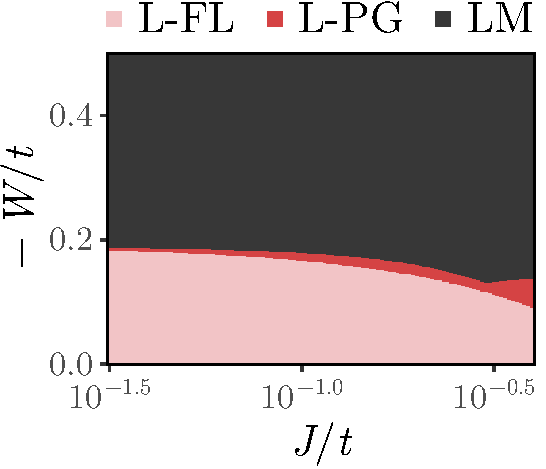
\includegraphics[width=0.31\linewidth, height=2.45cm]{phaseDiagram.pdf}
    \includegraphics[width=0.67\linewidth]{SF-DOS.pdf}
    \caption{Left: Phase diagram of impurity model at strong coupling in $U$ in terms of competing dimensionless Kondo ($J/t$) and bath correlation ($W/t$) couplings. A pseudogap phase (red, PG) is observed between the local Fermi liquid (pink, LFL) and local moment (black, LM) phases. Center: $k-$space resolved spin-spin correlation $\chi_s(d,{\bf k}) = \braket{{\bf S}_d\cdot{\bf S}_{\bf k}}$ in the pseudogap phase of the impurity model. Antinodal regions are observed to decouple from Kondo screening of the impurity. Right: Upon tiling, this leads to a $k-$space resolved antinodal gap in the electronic density of states of the lattice model, corresponding to Luttinger surfaces of zeros.}
    \label{spinCorr}
\end{figure}
\par\noindent\textit{Pseudogapping transition from Kondo breakdown.} A detailed picture of Kondo breakdown in the large $U$ phase of $H_\text{aux}$ is obtained from a scaling analysis of the ${\bf k}$-resolved Kondo coupling \(J^{(j)}_{{\bf k}_1, {\bf k}_2}\) using the 
unitary renormalisation group (URG) method \cite{anirbanurg1} (see \cite{suppmat} for details)
\begin{equation}\begin{aligned}\label{KondoRGequation}
	\Delta J^{(j)}_{{\bf k}_1, {\bf k}_2} = -\sum_{{\bf q} \in \text{PS}} \frac{J^{(j)}_{{\bf k}_2,{\bf q}} J^{(j)}_{{\bf q},{\bf k}_1} + 4J^{(j)}_{{\bf q}, {\bf \bar q}} W_{{\bf \bar q}, {\bf k}_2, {\bf k}_1, {\bf q}}}{\omega - \frac{1}{2}|\varepsilon_j| + J^{(j)}_{{\bf q}}/4 + W_{{\bf q}}/2}~,
\end{aligned}\end{equation}
where \(\varepsilon_j\) is the energy of the shell being decoupled at the \(j^\text{th}\) step, the sum is over all momentum states \({\bf q}\) in the particle sector (PS) of the energy shell \(\varepsilon_j\) (i.e., all states occupied at \(T=0\) and in the absence of any quantum fluctuations), and  \({\bf \bar q} = {\bf q} + {\boldsymbol \pi}\) is the particle-hole transformed state associated with ${\bf q}$. The bath interaction coupling $W_{{\bf \bar q}, {\bf k}_2, {\bf k}_1, {\bf q}}$ is found to be marginal under these transformations. While the complexity of the RG equation for $J_{{\bf k}_1, {\bf k}_2}$ (eq.\eqref{KondoRGequation}) is clarified through a detailed numerical evaluation whose results are discussed below, its structure permits the broad conclusion that the frustration of Kondo screening due to charge fluctuations (arising for attractive bath interactions $W<0$) lead to the Mott metal-insulator transition~\cite{Mukherjee_2023}.

Upon tuning the ratio of the bath and Kondo interactions ($W/J$) from zero to negative values (see phase diagram in Fig.\ref{spinCorr}(left)), we observe that the following phases are emergent in the impurity model from the competition between the competing $J$ and $W$ couplings in eq.~\eqref{KondoRGequation}- (i) for $W/J<(W/J)_{\text{PG}}$, a local Fermi liquid phase (where the entirety of the Fermi surface participates in Kondo screening), (ii) for $\frac{W}{J} \in [(\frac{W}{J})_{\text{PG}}, (\frac{W}{J})_c]$, a local PG phase where disconnected parts of the Fermi surface around the node participate in Kondo screening, and (iii) a local moment phase for $\frac{W}{J} > (\frac{W}{J})_c$, where the impurity remains unscreened at low-energies. These can be visualised from $k-$space resolved spin correlations $\chi_s(d,{\bf k}) = \braket{{\bf S}_d\cdot{\bf S}_{\bf k}}$; see Fig.\ref{spinCorr}(center) for $\chi_s(d,{\bf k})$ in the PG. The values $(W/J)_{\text{PG}}$ and $(W/J)_c$ are hence defined as the entry into and exit from the PG phase. Upon mapping to the lattice model via tiling, we observe that the $T=0$ Mott transition of the 2D Hubbard-Heisenberg model proceeds from Fermi liquid to Mott insulator through an intervening PG phase with a partially gapped Fermi surface (i.e., a vanishing electronic density of states around the antinodal regions, Fig.\ref{spinCorr}(right)). We now lay out the mechanism for the formation of the PG. 

\begin{figure}[htpb]
    \centering
    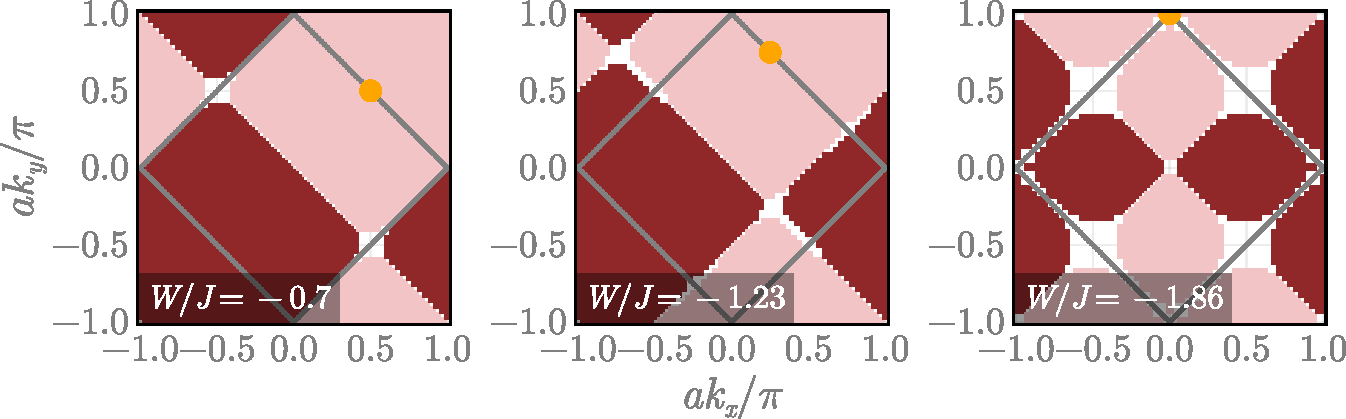
\includegraphics[width=\linewidth]{zerosFlow.pdf}
    \caption{Left, Right and Center: Decoupling of $J_{{\bf k}, {\bf k'}}$ (positive, negative and zeros shown in yellow, purple and green respectively), with ${\bf k}$ (grey circle) corresponding to the node, antinode and a point mid-way between them on the top right arm of the Fermi surface respectively. This is seen via the appearance of zeros (green patches) of $J_{{\bf k}, {\bf k'}}$ for ${\bf k'}$ initially on the nodal regions of adjacent arms, and their subsequent progression towards the antinodes. The decoupling 
    ends with the onset of the pseudogap.
    }
    \label{rgProgression}
\end{figure}

\par\noindent\textit{Unraveling of Kondo screening.} 
As shown in Fig.\ref{rgProgression}, the $k-$space anisotropic nature of the Kondo breakdown process 
can be visualised in terms of zeros of $J_{{\bf k}_N, {\bf k}}$, involving spin-flip scattering between the node ${\bf k}_N = (\pi/2, \pi/2)$  and a general wavevector ${\bf k}$. 
At $W/J=0$, $J_{{\bf k}_N, {\bf k}}$ vanishes if ${\bf k}$ is either any of the antinodes or adjacent nodes. Tuning $W/J$ towards $(W/J)_{\text{PG}}$ leads to an unraveling of Kondo screening: $J_{{\bf k}_N, {\bf k}}$ for ${\bf k}$ close to the adjacent nodes turn RG irrelevant first, and a patch of zeros subsequently appears in $J_{{\bf k}_N, {\bf k}}$ around this point (Fig.\ref{rgProgression}(left)). Tuning $W/J$ further extends the patch of zeros in $J_{{\bf k}_1, {\bf k}_2}$ for ${\bf k}_{1}$ lying between a given node and the nearest antinodes (Fig.\ref{rgProgression}(center) and (right)), visualising a systematic decoupling of $J_{{\bf k}_1, {\bf k}_2}$ connecting adjacent quadrants of the Brillouin zone quadrants. Precisely at $W/J=(W/J)_{\text{PG}}$, the antinode joins this connected region of zeros in $J_{{\bf k}_1, {\bf k}_2}$, marking (within our numerical precision) to the decoupling of the antinodes from all other points in the neighbourhood of the Fermi surface. This is an interaction-driven Lifshitz transition of the Fermi surface, and marks entry into a PG phase possessing Fermi arcs~\cite{WuFerrero2018}. Importantly, it coincides with an emergent two-channel Kondo (2CK) impurity model, where each channel corresponds to a pair of Fermi arcs on opposite faces of the conduction bath Fermi surface. The 2CK nature of the PG is guaranteed by the symmetry: 
$J_{{\bf k},{\bf k'}}= -J_{{\bf k}+{\bf Q},{\bf k'}}=-J_{{\bf k},{\bf k'}+{\bf Q}}$, where ${\bf Q} = (\pi,\pi)$. The PG expands by shrinking these disconnected Fermi arcs towards the respective nodes, leading to nodal metals whose disappearance marks the Mott transition. 
\par\noindent\textit{{\bf k}-resolved dynamical spectral weight transfer.}
As shown in Fig.\ref{chargeCorr}(left), strong charge fluctuations develop between the nodal and antinodal regions of the Fermi surface in the PG regime, removing low-energy spectral weight from the antinodes to higher energies and leading to their selecting gapping. Accordingly, the PG coincides with the appearance of poles of the lattice model self-energy $\Sigma ({\bf k},\omega=0)$ near the antinodes; these poles approach the nodes upon tuning towards the Mott transition (Fig.\ref{chargeCorr}(right)). This mirrors the coalescing of self-energy poles at zero frequency in the underlying impurity model~\cite{suppmat}. 
\begin{figure}
    \centering
    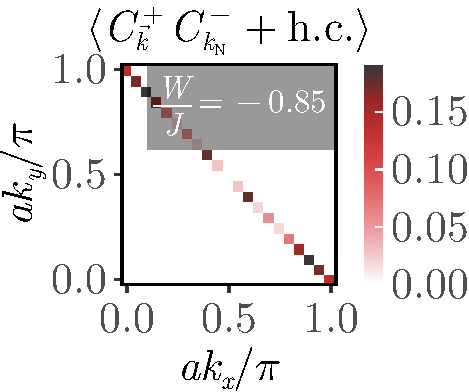
\includegraphics[width=0.49\linewidth]{cfnode-2.pdf}
    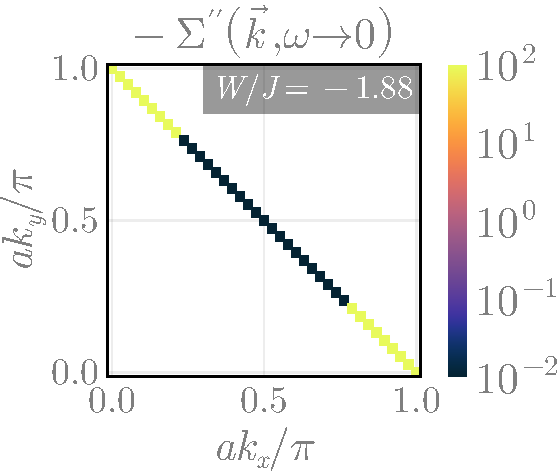
\includegraphics[width=0.49\linewidth]{selfEnergyKspace-3.pdf}
    \caption{Left: Enhanced charge isospin correlations $\chi_c({\bf k}_1, {\bf k}_2) = \braket{c^\dagger_{{\bf k}_1\uparrow}c^\dagger_{{\bf k}_1\downarrow}c_{{\bf k}_2\downarrow}c_{{\bf k}_2\uparrow} + \text{h.c.}}$ between the nodal and antinodal regions, signalling Kondo breakdown in the pseudogap phase of the impurity model. Right: In turn, the breakdown leads to the gapping of the antinodal regions in the lattice model, seen from the appearance of poles in the imaginary part of the self-energy.}
    \label{chargeCorr}
\end{figure}

\par\noindent\textit{Non-Fermi liquid nature of the pseudogap.}
In the PG regime $|W/J|_{\text{PG}} < |W/J| < |W/J|_{c}$, the nature of the gapless Fermi arcs is observed to change dramatically. We have already argued that the low-energy dynamics of these gapless Fermi arcs are governed by an underlying two-channel Kondo (2CK) impurity model~\cite{Tsvelick_weigmann_mchannel_1985,emery_kivelson}.
The excitations of the 2CK exhibit a separation of spin, charge and channel quantum numbers~\cite{affleck1992}, with gapless excitations carrying only the spin quantum number. Previous works show that the impurity self-energy of such a two-channel Kondo model displays marginal Fermi liquid (MFL) behaviour~\cite{Coleman_tsvelik,Schofield1997,Patra2023MCK} with real and imaginary parts of the self-energy as $\Sigma^{\prime} \sim \omega\ln\omega, \Sigma^{\prime\prime}\sim-\omega$. This gives rise~\cite{varma2002singular} to a linear scattering rate \(\Gamma \sim \omega\), and a logarithmically vanishing quasiparticle residue $Z_\text{imp}(\omega) 
\sim (c - \ln \omega)^{-1}$ (where \(c\) is a constant). 
This is consistent with the rapid fall of the impurity quasiparticle residue $Z_\text{imp}$ (Fig.\ref{channelDecoupling}(left)) from finite values in the Fermi liquid phase to vanishingly small values in the PG. The inset of Fig.\ref{channelDecoupling}(left) shows the emergence of increasingly uncompensated local magnetic moments upon traversing the PG phase. 

\begin{figure}
    \centering
    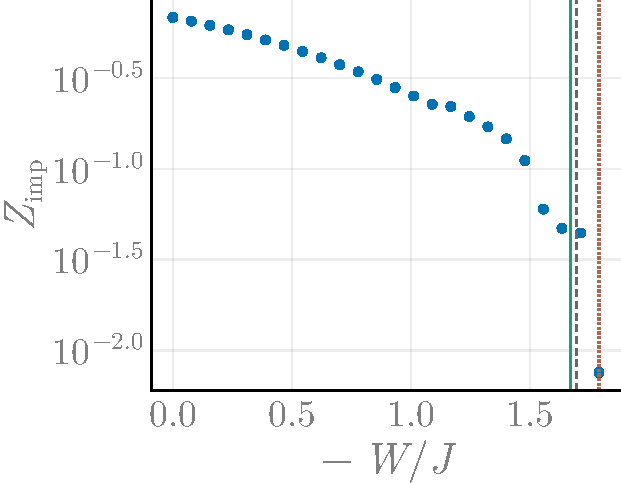
\includegraphics[width=0.49\linewidth]{localQPResidue.pdf}
    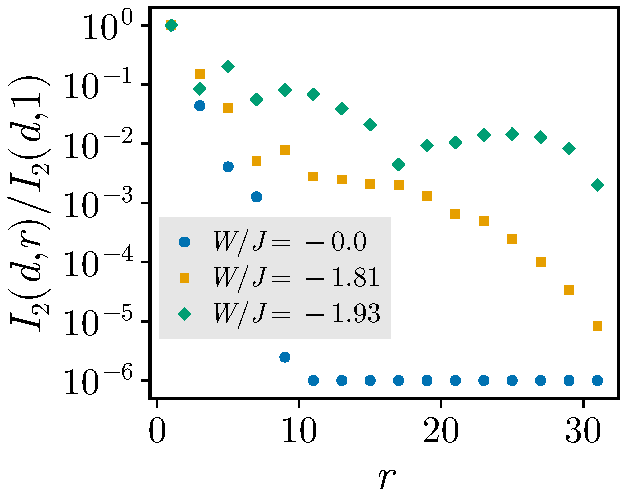
\includegraphics[width=0.49\linewidth]{I2-di_69-2000.pdf}
    \caption{Left: Suppression of quasiparticle residue as the impurity model is tuned towards the Mott transition. An initial drastic fall observed for $W/J \lesssim (W/J)_\text{PG}$, signalling the destruction of the Fermi liquid with unraveling of Kondo screening. A second drastic fall is observed close to the Mott transition due to a divergent self-energy. Inset shows the growth of unscreened impurity magnetic moment in the pseudogap phase. 
    Right: Mutual information $I_{2}(d,r)$ between the impurity spin and conduction bath local spins as a function of the distance {\bf r} between them. $I_{2}(d,r)$ decays exponentially in the Fermi liquid phase (blue), but show long-ranged behaviour in the non-Fermi liquid phase (green, yellow). The range of the entanglement is seen to grow yet larger particularly close to the transition (green).
    }
    \label{channelDecoupling}
\end{figure}

\par\noindent\textit{Evolution of the pseudogapped non-Fermi liquid.} Very close to the transition, the excitations of the marginal Fermi liquid are replaced by those of a Hatsugai-Kohmoto model~\cite{Baskaran1991,Hatsugai1992}. This insight is obtained from a perturbation-theoretic treatment of the RG fixed point Hamiltonian of the impurity model for $W/J\lesssim (W/J)_{\text{PG}}$, by considering the effects of a small fixed point Kondo scattering probability \(J^*\) in the backdrop of a larger bath interaction parameter \(|W|\). This yields the HK model~\cite{Baskaran1991,Hatsugai1992} as the singular part of the effective Hamiltonian arising from forward scattering processes (details in Appendix~\ref{hkmDerivation}):
\begin{equation}\begin{aligned}\label{HKModel}
	\Delta \tilde H_{{\bf q}_1 = {\bf q}_2} = \sum_{{\bf q},\sigma}\epsilon_{{\bf q}}{n}_{{\bf q},\sigma} + u\sum_{{\bf q}, \sigma}n_{{\bf q} \sigma} n_{{\bf q} \bar\sigma}~,
\end{aligned}\end{equation}
where the number operator \(n_{{\bf q} \sigma} = \phi^\dagger_{{\bf q}, \sigma} \phi_{{\bf q}, \sigma}\) pertains to emergent fermionic relative modes $\phi_{{\bf q}, \sigma}$ that are shifted by an excitation momentum \({\bf q}\) away from the nodal point \({\bf N}_1 = \left(\pi/2, \pi/2\right)\) and its 
partner \({\bf N}_1 + {\bf Q}_1 = \left(-\pi/2, -\pi/2\right)\). The kinetic energy \(\epsilon_{\bf q}\) and interaction energy \(u\sim J^{2}/W\) are dispersion and Kondo scales renormalised by conduction bath correlations~\cite{suppmat}.

Consequently, the resulting non-Fermi liquid metal of the lattice model involves long-lived excitations of multiple \({\bf k}\)-states, and manifest in the form of 
a divergent one-particle self-energy at the non-interacting Fermi surface~\cite{Phillips2020}:
	$\Sigma_{{\bf q}}(\omega) = -\frac{u^2/4}{\omega - \epsilon_{\bf q}}$, such that $\Sigma_{\epsilon_{\bf q}=0}(\omega \to 0)  \to \infty$. This zero-frequency self-energy pole 
presages the transition into a Mott insulating phase, where it marks a hard gap in the spectral function for charge excitations. This is consistent with our findings for the lattice (Fig.\ref{chargeCorr}(right)) and impurity self-energies~\cite{suppmat}. Further, for small but non-zero values of \(\omega - \epsilon_{\bf k}\), we obtain the quasiparticle residue \(Z_\text{imp} \sim \omega^2/U^2 \), i.e., a faster vanishing of $Z_{imp}$ compared to the MFL. This explains the sharp fall in $Z_\text{imp}$ observed precisely at the transition (Fig.\ref{channelDecoupling}(left)). The scattering rate precisely at the Fermi surface \(\omega=\epsilon_{\bf k}\) diverges, \(\Gamma \sim U^2\delta(\omega - \epsilon_{\bf k})\), in contrast to \(\Gamma \sim \omega\) observed for the MFL.
\par\noindent\textit{Non-local nature of the pseudogap.}
In Fig.\ref{channelDecoupling}(right), mutual information between the impurity spin and conduction bath sites are observed to undergo a crossover within the PG, from short-ranged behaviour at its onset to long-ranged behaviour as the Mott transition is approached. Similar long-ranged behaviour of spin-flip correlations is also observed between the impurity and bath sites~\cite{suppmat}. This is further evidence of the breakdown of local Kondo screening, and resulting Landau quasiparticle excitations. 
This implies that the observed Mott transition lies well beyond the paradigm of local quantum criticality~\cite{Si2001}: the non-Fermi liquid Fermi arcs of the PG phase display increasingly critical behaviour close to the transition, with dynamics that cannot be described by local quantum fluctuations, and excitations that become truly long-ranged. Additionally, we observe that the nodal metal possesses pairing fluctuations~\cite{suppmat} that can be rendered dominant upon doping~\cite{Phillips2020}.
\par\noindent\textit{Conclusions.} We find compelling evidence that the Mott transition involves continuous passage through a PG phase possessing an increasingly singular, non-local nodal non-Fermi liquid metal, and the onset of long-ranged entanglement at criticality. The evolution of this singular PG phase with doping 
deserves attention.
\par\noindent\textit{Acknowledgments.}
AM thanks IISER Kolkata for funding through a JRF and SRF. S Lal thanks the SERB, Govt. of India for funding through MATRICS Grant MTR/2021/000141 and Core Research Grant CRG/2021/000852.
\bibliography{tilingProject}% Produces the bibliography via BibTeX.

\appendix

\section{Appendixes}
\paragraph*{Luttinger's theorem in the presence of Luttinger surfaces.} One can also ask whether Luttinger's theorem is satisfied in our model in the presence of Luttinger surfaces. It has been shown that particle-hole symmetric systems always satisfy a generalised Luttinger's theorem~\cite{seki2017topological}, where the Fermi volume $V_L$ is represented as the difference in the number of poles and zeros, of the single-particle Greens function, that are enclosed by the Fermi surface~\cite{seki2017topological}. This holds true even in the presence of a divergent self-energy~\cite{Phillips2013}. Since our model is always at half-filling, Luttinger's theorem is always satisfied. 

The way it works out (despite the presence of Luttinger surfaces) is as follows. We need only show that the number of occupied states below the chemical potential remains unchanged across the first Lifshitz transition. Before the transition, the presence of gapless excitations ensures that the Fermi surface is singly-occupied on average. Inside the pseudogap, the gapless $k-$states continue to contribute one pole on average to the Luttinger count, while the gapping out of certain $k-$states leads to a rearrangement of their spectrum: doubly-occupied states on the Luttinger surfaces become more favourable compared to the singly-occupied states (due to the attractive $W$-interaction). Owing to particle-hole symmetry, these states are degenerate with the zero occupancy states, so that on average, a single state is again occupied. This ensures that the number of occupied states (and hence the number of occupied poles) remains unchanged across the transition. The same argument works for the Mott insulator, where the entire Fermi surface gets replaced by a Luttinger surface.

\paragraph*{Tiling towards a Hubbard-Heisenberg model with an embedded extended SIAM}
We give more details here regarding the construction of the lattice model from the impurity model. As mentioned in the manuscript, the lattice-embedded impurity model is of the form $H({\bf r}_d) = H_\text{imp} + H_\text{cbath} + H_\text{imp-cbath}$, where $H_\text{imp}$ is the impurity part:
\begin{equation}\begin{aligned}\label{onsiteHamiltonian}
	H_\text{imp} = -\frac{U}{2}\left(\hat n_{{\bf r}_d \uparrow} - \hat n_{{\bf r}_d \downarrow} \right)^2 - \eta\sum_\sigma \hat n_{{\bf r}_d\sigma}~,
\end{aligned}\end{equation}
\(\mathcal{H}_\text{cbath}\) is the conduction bath part:
\begin{equation}\begin{aligned}\label{bathHamiltonian}
	{H}_\text{cbath} = -\frac{1}{\sqrt\mathcal{Z}}t\sum_{\left<{\bf r}_i, {\bf r}_j\right>\neq{\bf r}_d;\sigma}\left(c^\dagger_{{\bf r}_i,\sigma}c_{{\bf r}_j,\sigma} + \text{h.c.}\right) - \\
    \frac{1}{2 \mathcal{Z}}W\sum_{{\bf z}\in\text{NN}({\bf r}_d)}\left(\hat n_{{\bf z}, \uparrow} - \hat n_{{\bf z}, \downarrow}\right)^2 - \mu \sum_{{\bf r}_i \neq {\bf r}_d}\hat n_{{\bf r}_i,\sigma}~,
\end{aligned}\end{equation}
and ${H}_\text{imp-cbath}$ is the impurity-bath hybridisation:
\begin{equation}\begin{aligned}\label{interactionHamiltonian}
	{H}_\text{imp-cbath} = \frac{J}{\mathcal{Z}}\sum_{\sigma,\sigma^\prime}\sum_{{\bf z}\in\text{NN}({\bf r}_d)} {\bf S}_{{\bf r}_d}\cdot{\boldsymbol \tau}_{\sigma,\sigma^\prime}c^\dagger_{{\bf z},\sigma}c_{{\bf z},\sigma^\prime} \\
    - \frac{V}{\sqrt{\mathcal{Z}}}\sum_{\sigma} \sum_{{\bf z}\in\text{NN}({\bf r}_d)}\left(c^\dagger_{{\bf r}_d,\sigma} c_{{{\bf z}},\sigma} + h.c.\right)~.
\end{aligned}\end{equation}
In this model, ${\bf r}_d$ is the position of the impurity site, and \(\left<{\bf r}_i, {\bf r}_j\right>\neq {\bf r}_d\) indicates that the sum is over all nearest-neighbour pairs of sites avoiding the impurity site \({\bf r}_d\). \(\boldsymbol \tau = \left( \tau_x, \tau_y, \tau_z \right) \) is the vector of Pauli matrices. \(\sigma\) and \(\sigma^\prime\) can be \(\pm 1\) and represent up and down configurations.

The tiled Hamiltonian can be obtained as 
\begin{equation}\begin{aligned}
	\mathcal{H}_\text{tiled} = \mathcal{T}[H({\bf r}_d)]
    % \sum_{{\bf r}}T^\dagger({\bf r} - {\bf r}_d)H({\bf r}_d)T({\bf r} - {\bf r}_d)~,
\end{aligned}\end{equation}
where the $\mathcal{T}[H] = \sum_{{\bf r}}T^\dagger({\bf r} - {\bf r}_d)HT({\bf r} - {\bf r}_d)$ represents the symmetrisation/tiling procedure, and the action of the many-body translation operators $T^\dagger({\bf a})$ on a general operator are defined as
\begin{equation}\begin{aligned}
T^\dagger({\bf a}) \mathcal{O}\left({\bf r}_1, {\bf r}_2,\ldots\right)T({\bf a}) = \mathcal{O}\left({\bf r}_1 + {\bf a}, {\bf r}_2 + {\bf a},\ldots\right)~.
\end{aligned}\end{equation}

We consider the effect of the translation operations on each part of the Hamiltonian:
\begin{equation}\begin{aligned}
	&\mathcal{T}\left[{H}_\text{cbath}({\bf r}_d, {\bf z})\right] = -\frac{(N-2)t}{\sqrt\mathcal{Z}}\sum_{\left<{\bf r}_i, {\bf r}_j\right>;\sigma}\left(c^\dagger_{{\bf r}_i,\sigma}c_{{\bf r}_j,\sigma} + \text{h.c.}\right) \\
    &- \frac{1}{2}W\sum_{\bf r}\left(\hat n_{{\bf r} , \uparrow} - \hat n_{{\bf r} , \downarrow}\right)^2 - \mu (N-1) \sum_{{\bf r}}\hat n_{{\bf r},\sigma}~,\\
	&\mathcal{T}\left[{H}_\text{imp}\right] = -\frac{U}{2}\sum_{{\bf r}}\left(\hat n_{{\bf r} \uparrow} - \hat n_{{\bf r} \downarrow} \right)^2 - \eta\sum_{{\bf r},\sigma} \hat n_{{\bf r}\sigma}~,\\
    &\mathcal{T}\left[{H}_\text{imp-cbath}\right]\\
     &=\sum_{\left< {\bf r}_i, {\bf r}_j\right>}\left[\frac{2}{\mathcal{Z}}J {\bf S}_{{\bf r}_i}\cdot{\bf S}_{{\bf r}_j} - \frac{2}{\sqrt\mathcal{Z}}V \sum_{\sigma}\left(c^\dagger_{{\bf r}_i,\sigma} c_{{{\bf r}_j},\sigma} + h.c.\right)\right]~.
\end{aligned}\end{equation}
We have defined \({\bf S}_{{\bf r}_j} =\sum_{\sigma,\sigma^\prime} {\boldsymbol \tau}_{\sigma,\sigma^\prime}c^\dagger_{{\bf z},\sigma}c_{{\bf z},\sigma^\prime}\) as the local spin operator. While constructing the tiled Hamiltonian, we have added extra copies of the non-interacting Hamiltonian \(\mathcal{H}_\text{cbath-nint} = -\frac{1}{\sqrt\mathcal{Z}}t\sum_{\left<{\bf r}_i, {\bf r}_j\right>;\sigma}\left(c^\dagger_{{\bf r}_i,\sigma}c_{{\bf r}_j,\sigma} + \text{h.c.}\right) - \mu \sum_{{\bf r}}\hat n_{{\bf r},\sigma}\) for the conduction bath (this results in the factors of \(N-2\) and \(N-1\) in front of the first and third terms).

Upon removing these repeated terms, the result of the tiling operations is a Hubbard-Heisenberg model, of the form
\begin{equation}\begin{aligned}
	\mathcal{H}_\text{HH} &= -\frac{1}{\sqrt\mathcal{Z}}\tilde t\sum_{\left<{\bf r}_i, {\bf r}_j\right>;\sigma}\left(c^\dagger_{{\bf r}_i,\sigma}c_{{\bf r}_j,\sigma} + \text{h.c.}\right) - \tilde \mu \sum_{{\bf r}}\hat n_{{\bf r},\sigma} \\
    &+ \frac{1}{\mathcal{Z}}\tilde J\sum_{\left< {\bf r}_i, {\bf r}_j\right>}{\bf S}_{{\bf r}_i}\cdot{\bf S}_{{\bf r}_j} - \frac{1}{2}\tilde U\sum_{\bf r}\left(\hat n_{{\bf r} , \uparrow} - \hat n_{{\bf r} , \downarrow}\right)^2  ~,
\end{aligned}\end{equation}
where the tilde symbol indicates that the parameters are for the lattice model (and not the auxiliary model). By comparing the tiled model and the general lattice model, the lattice model parameters and the auxiliary model parameters can be mapped to each other:
\begin{equation}\begin{aligned}\label{couplingsMappings}
	\tilde t = t+2V,~~ \tilde U = U + W, ~ ~ \tilde \mu = 2\mu + \eta,~ ~ \tilde J = 2J~.
\end{aligned}\end{equation}
In summary, the appropriate method for reconstructing the lattice model Hamiltonian is therefore
\begin{equation}\begin{aligned}\label{tilingPrescriptionFinal}
	\mathcal{H}_\text{tiled} &= \sum_{{\bf r}}\mathcal{H}_\text{aux}({\bf r}) - N\mathcal{H}_\text{cbath-nint}~,
\end{aligned}\end{equation}
where we replaced \(N-3\) with \(N\) assuming a large number of sites. Using this, the extended-SIAM gets ``expanded" into a Hubbard-Heisenberg model.
\end{document}
